\begin{frame}
    \frametitle{Pregunta 1}

    Mencione todos los algoritmos de clustering y sus variantes implementados como parte de la aplicación.
    Comente sobre la implementación de los mismos, incluyendo una breve descripción de cualquier biblioteca utilizada.

\end{frame}

\begin{frame}
    \frametitle{Pregunta 1}

    \begin{itemize}
        \item K-Means
        %        \begin{verbatim}
        %        sklearn.cluster.KMeans(n_clusters, random_state, init=\'k-means++\', ...)
        %        \end{verbatim}

        \item HDBSCAN
        %        \begin{verbatim}
        %        hdbscan.HDBSCAN(min_cluster_size, \ldots)
        %        \end{verbatim}

        \item Gaussian Mixture Model
        %        \begin{verbatim}
        %        sklearn.mixture.GaussianMixture(n_components, random_state, covariance_type='full', max_iter=100, init_params='kmeans', \ldots)
        %        \end{verbatim}

        \item Spectral Clustering
        %        \begin{verbatim}
        %        sklearn.cluster.SpectralClustering(n_clusters, random_state, \ldots)
        %        \end{verbatim}
        %
        \item Affinity Propagation
        %        \begin{verbatim}
        %        sklearn.cluster.AffinityPropagation(damping=0.5, max_iter=200, convergence_iter=15, \ldots)
        %        \end{verbatim}
    \end{itemize}

\end{frame}

\begin{frame}
    \frametitle{Pregunta 2}

    Mencione detalles de la librería de Python implementada, incluyendo las clases principales que la componen y cómo puede ser utilizada y expandida.

\end{frame}

\begin{frame}
    \frametitle{Pregunta 2}

    \begin{figure}[!h]
        \centering
        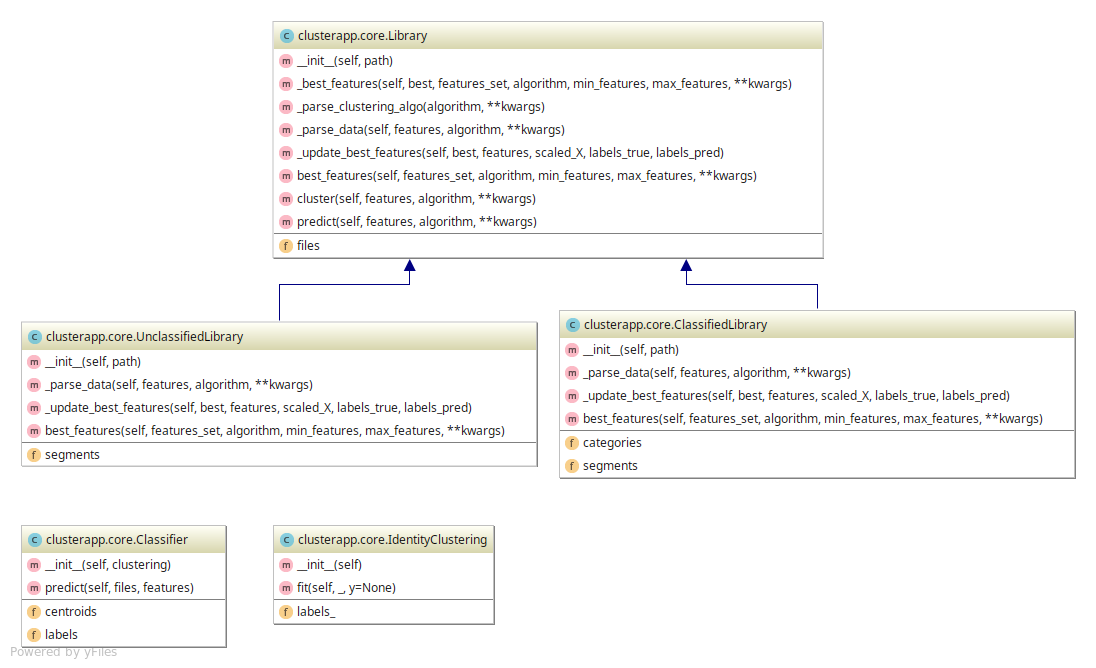
\includegraphics[width=0.95\textwidth]{core-library-uml.png}
    \end{figure}

\end{frame}

\begin{frame}
    \frametitle{Pregunta 3}

    En los conjuntos de datos donde una misma especie puede presentar distintos tipos de vocalizaciones, ¿qué resultados se obtienen para los algoritmos de clustering cuando se toman las especies y no los tipos de vocalizaciones específicos como categoría?
    Compare estos resultados con los presentados en el trabajo.

\end{frame}

\begin{frame}
    \frametitle{Pregunta 3}

    \begin{figure}[!h]
        \centering
        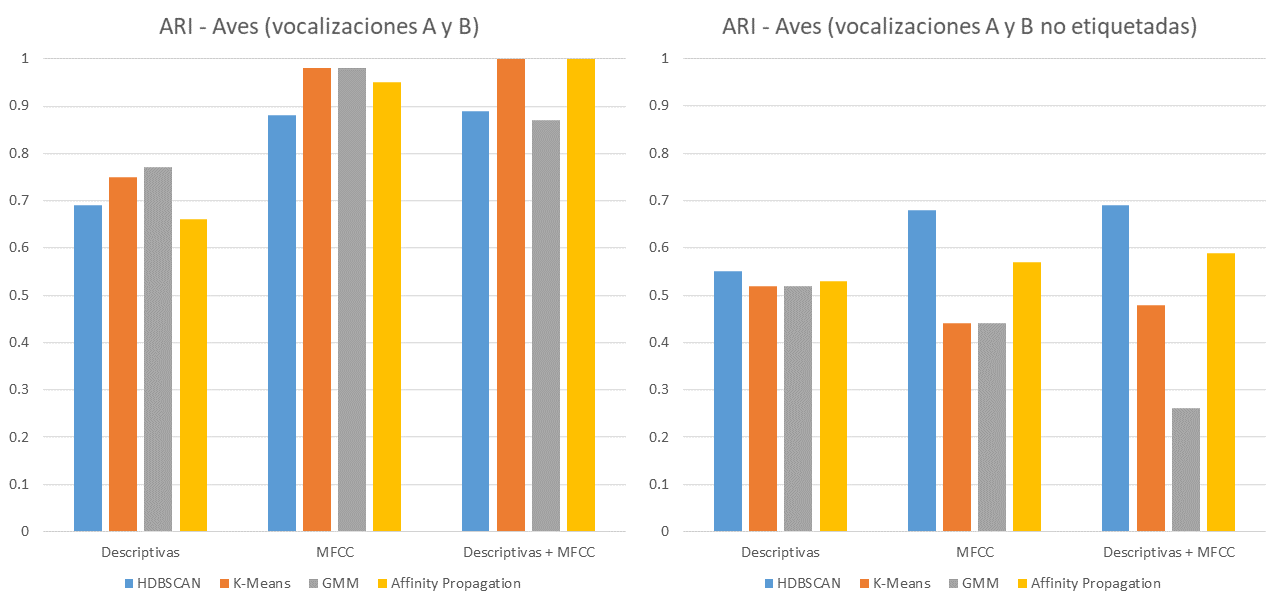
\includegraphics[width=\textwidth]{question3.png}
    \end{figure}

\end{frame}

\begin{frame}
    \frametitle{Pregunta 3}
    \framesubtitle{Conjunto de datos}

    \begin{figure}[!h]
        \centering
        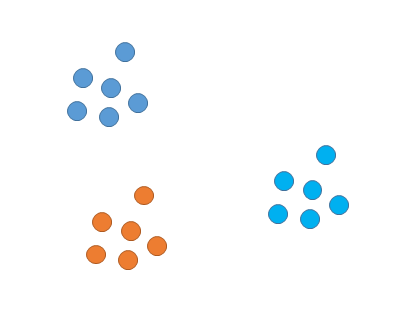
\includegraphics[width=0.7\textwidth]{question3-dataset.png}
    \end{figure}

\end{frame}

\begin{frame}
    \frametitle{Pregunta 3}
    \framesubtitle{Algoritmo supervisado}

    \begin{figure}[!h]
        \centering
        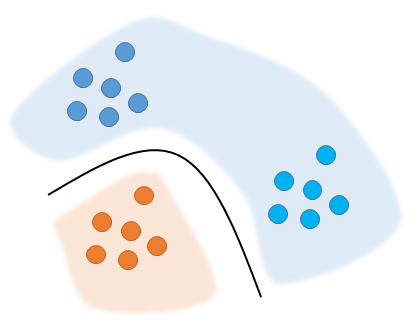
\includegraphics[width=0.7\textwidth]{question3-supervised.png}
    \end{figure}

\end{frame}

\begin{frame}
    \frametitle{Pregunta 3}
    \framesubtitle{Algoritmo no supervisado}

    \begin{figure}[!h]
        \centering
        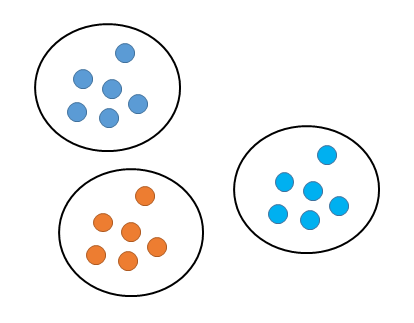
\includegraphics[width=0.7\textwidth]{question3-unsupervised.png}
    \end{figure}

\end{frame}
